\documentclass[10pt, oneside]{article} 
\usepackage{amsmath, amsthm, amssymb, calrsfs, wasysym, verbatim, bbm, color, graphics, graphicx, geometry}
\usepackage[most]{tcolorbox}
\usepackage{xcolor}
\usepackage{framed}
\colorlet{shadecolor}{blue!15}
\graphicspath{ {./} }

\geometry{tmargin=.75in, bmargin=.75in, lmargin=.75in, rmargin = .75in}  

\newcommand{\R}{\mathbb{R}}
\newcommand{\C}{\mathbb{C}}
\newcommand{\Z}{\mathbb{Z}}
\newcommand{\N}{\mathbb{N}}
\newcommand{\Q}{\mathbb{Q}}
\newcommand{\Cdot}{\boldsymbol{\cdot}}

\newtheorem{thm}{Theorem}
\newtheorem{defn}{Definition}
\newtheorem{conv}{Convention}
\newtheorem{rem}{Remark}
\newtheorem{lem}{Lemma}
\newtheorem{cor}{Corollary}
\newtheorem{exa}{Example}


\title{Clase \# 4: Cinem\'atica de los fluidos [MF100]}
\author{\textbf{Luis Alejandro Morales}\\ \vspace{0.4cm} Profesor Asistente \\ Universidad Nacional de Colombia-Bogot\'a\\Facultad de Ingenier\'ia \\ Departamento de Ingenieria Civil y Agr\'icola}
\date{Periodo 2022-II}

\begin{document}

\maketitle
\tableofcontents

\vspace{.25in}

\section{Descripci\'on Lagrangiana y Euleriana del movimiento de un fluido}
%La \emph{cinematica de los fluidos} describe como los fluidos fluyen y como se mueven. Dicha descripcion es posible bajo dos diferentes metodos: \textbf{descripci\'on Lagrangiana} y \textbf{descripci\'on Euleriana}
%
%\subsection{Descripci\'on Lagrangiana}
%Esta descripcion consiste en analizar el moviento individual de diferentes particulas de fluido, con el fin de determinar su posicion y su velocidad en un instante determinado. Fue planteado por el matematico Italiano Joseph Louis Lagrange (1736-1813). Esta descripcion es facil de utilizar por el ejemplo en el analisis del movimiento de bolas de billar. Sin embargo en el caso de un fluido, la definicion de una particula y su interaccion con otras es mas complejo teniendo en cuenta que el fluido es un continuo y este se deforma durante el movimiento. A pesar de esto, esta descripci\'on es utilizada en el an\'alisis del movimiento de contaminantes y en la visualizaci\'on de fluidos.  
%
%\subsection{Descripci\'on Lagrangiana}
%
%\subsection{Descripci\'on Euleriana y Lagrangiana}
Existen dos aproximaciones para analisar la cinematica de los fluidos. La primera se centra en el analisis de los campos de flujo y es conocido como el metodo \textbf{Euleriano}.  En el metodo euleriano, se calcula la presi\'on del campo de flujo $p(x,y,z,t)$  (e.g en un punto del espacio $x,y,z$ o section) mas no los cambios de presion que experimentar\'ia una part\'icula moviendose en el flujo. Aqui, la posicion del sistema de coordenadas es constante para un intervalo de tiempo (ver Figura~\ref{eulan}).
La segunda aproximaci\'on se centra en seguir particulas individualmente moviendose a traves del flujo, esto es conocido como el metodo \textbf{Lagrangiano}. En este, el sistema de coordenadas se mueve con el flujo. El metodo lagrangiano es mas apropiado para el analisis de solidos, mientras que el metodo euleriano esampliamente usado en mecanica de fluidos. 
En mediciones en fluidos, un sensor de presion introducido en un canal de laborario determina la presion del flujo en un punto ($x,y,z$) y en un instante ($t$) determinado. Dicha medicion es acorde con el metodo euleriano. De acuerdo con el metodo lagrangiano,  el mismo sensor arrojado al flujo y moviendose a la misma velocidad permitiria medir la presion de una particula que se mueve con el flujo.

\begin{figure}[h]
\centering
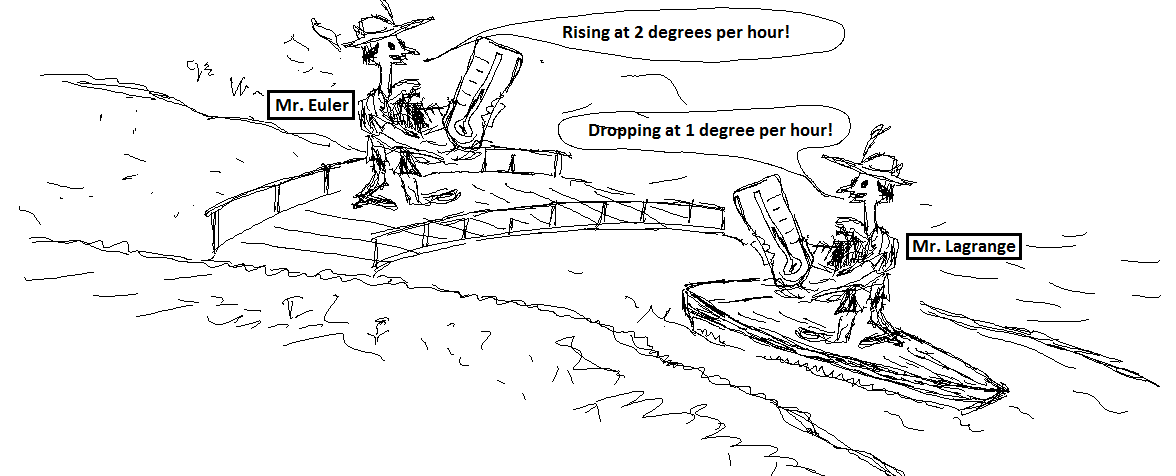
\includegraphics[width=8cm]{MaterialDerivative}
\caption{Sistema euleriano y lagrangiano (http://www.flowillustrator.com/fluid-dynamics/basics/lagrangian-eulerian-viewpoints.php)}
\label{eulan}
\end{figure}

\subsection{El campo de velocidad}
La   propiedad mas conocida de un flujo es el campo de velocidad $\vec{V}(x,y,z,t)$, de la cual se derivan otras propiedades. La velocidad es un vector en funcion de la posicion y del tiempo y por lo tanto tiene tres componentes escalares $u$, $v$ y $w$:
$$
\vec{V}(x,y,z)=u(x,y,z,t)\vec{i} + v(x,y,z,t)\vec{j} + w(x,y,z,t)\vec{k}
$$

\subsection{El campo de aceleracion}
El vector de aceleracion, $\vec{a}=\frac{d \vec{V}}{dt}$ es importante en flujos ssometidos a algun tipo de fuerza segun la segunda ley de Newton. El campo de aceleraci\'on de un fluido con respecto a un marco de referencia Euleriano, se define como:
$$
\vec{a}=\frac{d \vec{V}}{dt}
$$

Si tenemos una  $y=f(u)$ donde $u=g(x)$, $y$ es una funcion compuesta $y=f(g(x))$ y derivable en $x$. De acuerdo con la \textbf{regla de la cadena}, la $\frac{dy}{dx}=\frac{dy}{du} \frac{du}{dx}$. Aplicando dicha regla a la ecuacion anterior tenemos: 

$$
\vec{a}=\frac{\partial \vec{V}}{dt} + u\frac{\partial \vec{V}}{dx} + v\frac{\partial \vec{V}}{dy} + w\frac{\partial \vec{V}}{dz}
$$

La aceleracion de una particula de flujo expresada como una variable de campo es:
\begin{equation}
\vec a(x,y,z,t) = \frac{d \vec{V}}{dt} = \frac{\partial \vec{V}}{\partial t} + (\vec{V} \cdot \vec{\nabla})\vec{V}
\label{ace}
\end{equation}

donde $\vec{\nabla}$ es el \emph{operador de gradiente}, el cual se define en coordenadas cartesianas como:
$$
\nabla = \left( \frac{\partial}{\partial x} , \frac{\partial}{\partial y}, \frac{\partial}{\partial z} \right) = \vec{i}\frac{\partial}{\partial x} +\vec{j}\frac{\partial}{\partial y}  + \vec{k}\frac{\partial}{\partial z}
$$

Las componentes de vector de aceleracion en coordenadas cartesianas son:
$$
a_x = \frac{\partial u}{\partial t} + u\frac{\partial u}{\partial x} + v\frac{\partial u}{\partial y} + w\frac{\partial u}{\partial z} \\
a_y = \frac{\partial v}{\partial t} + u\frac{\partial v}{\partial x} + v\frac{\partial v}{\partial y} + w\frac{\partial v}{\partial z} \\ 
a_z = \frac{\partial w}{\partial t} + u\frac{\partial w}{\partial x} + v\frac{\partial w}{\partial y} + w\frac{\partial w}{\partial z}  
$$

En la ecuacion~\ref{ace}, el termino $\partial \vec{V}/\partial t$ es conocida como la \emph{aceleracion local} y es diferente de zero para flujo no permanente. El segundo termino, $(\vec{V} \cdot \vec{\nabla})\vec{V}$ es conocido como la \emph{aceleracion advectiva} o la \emph{aceleracion convectiva}. Esta \'ultimo explica el movimiento de las particulas (adveci\'on o convecci\'on) de una localizacion hacia otra en el fluido donde el campo de velocidades del fluido es diferente. Por ejemplo consideremos la salida de agua de una manguera cuyo orificio de salida se reduce gradualmente (ver figura~\ref{acel}). En el sistema Euleriano, el flujo es considerado permanente ya que las propiedades del flujo en cualquier punto del flujo no cambian con el tiempo. Sin embardo, las particulas cambian de velocidad y se aceleran a la salida de la manguera en la reduccion gradual. Por lo tanto, la aceleracion no es zero debido al termino de aceleracion advectiva en la ecuacion~\ref{ace}. Se puede concluir que el flujo puede ser considerado \emph{permanente} desde un marco de referencia \emph{Euleriano} y \emph{no permanente} desde un marco de referencia \emph{Lagrangiano} que se mueve con el fluido. 

% Fig 4-8 Cengel 
\begin{figure}[h]
\centering
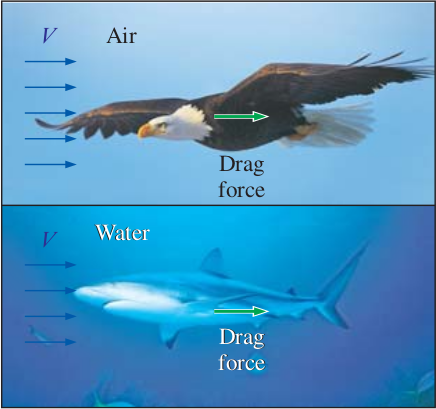
\includegraphics[width=8cm]{visco0}
\caption{Flujo a la salida de un manguera cuyo orificio se reduce y acelera el flujo a la salida.}
\label{acel}
\end{figure}

\subsection{Derivada material}
El operador de derivada total $d/dt$ en la ecuaci\'on~\ref{ace} es conocido como la \emph{derivada material}, $D/Dt$ la cual se deduce al seguir una  particula que se mueve con el campo de flujo. La derivada material se expresa como:
\begin{equation}
\underbrace{\frac{D}{Dt}}_{\substack{\text{Material} \\ \text{derivative}}} = \frac{d}{dt} = \underbrace{\frac{\partial}{\partial t}}_{\text{Local}} + \underbrace{(\vec{V} \cdot \vec{\nabla})}_{\text{Advective}}
\label{dma}
\end{equation}
Aplicando la ecuacion~\ref{dma} al campo de velocidades tenemos que $\frac{D\vec{V}}{Dt} = \frac{d\vec{V}}{dt}$ y se obtiene la ecuaci\'on~\ref{ace}, conocida tambien como la \emph{aceleracion material}.

La ecuacion~\ref{dma} puede ser aplicada a variables escalares como la presion:
$$
\frac{DP}{Dt}=\frac{dP}{dt}=\frac{\partial P}{\partial t} + (\vec{P} \cdot \vec{\nabla})\vec{V}
$$
la cual representa la tasa de cambio de la presion  de una particula que se mueve con el campo del flujo. 

\section{Patrones de flujo}
\subsection{Lineas de flujo}
Una \textbf{linea de flujo} es una curva que es tangente al vector de velocidad local en un instante de tiempo. Las lineas de flujo indican la direccion instantanea del movimiento del flujo. Esto quiere decir que en \emph{flujo no permanente} las lineas de flujo cambian con el tiempo. Si consideramos una longitud de arco infinitesimal $d\vec{r}=dx\vec{i}+dy\vec{j}+dz\vec{k}$ a lo largo de una linea de flujo donde $d\vec{r}$ es paralela al vector de velocidad local $\vec{V}=u\vec{i}+v\vec{j}+w\vec{k}$, por similaridad de triangulos $d\vec{r}$ debe ser proporcional a $\vec{V}$ (ver figura~\ref{strl}):
% Fig 4-16 Cengel 
\begin{figure}[h]
\centering
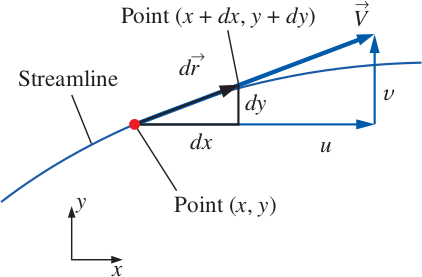
\includegraphics[width=8cm]{strl}
\caption{Linea de flujo y velocidad instantanea local en dos dimensiones.}
\label{strl}
\end{figure}
$$
\frac{dr}{V}=\frac{dx}{u}=\frac{dy}{v}=\frac{dz}{w}
$$
donde $dr$ es la magnitud de $d\vec{r}$ y $V$ es la magnitud de $\vec{V}$. En el plano $xy$, $(x,y)$, $(u,v)$, la siguiente ecuacion se obtiene: 
\begin{equation}
\left(\frac{dy}{dx}\right)_{a lo largo de la linea flujo} = \frac{v}{u}
\label{lnf}
\end{equation}
Conociendo el campo de velocidades, la ecuacion~\ref{lnf} puede ser resuelta analitica o numericamente pero en cualquier caso una constante de integracion es necesaria lo que daria lugar a una familia de curvas (lineas de flujo).

\subsection{Trayectorias de corriente}
Una \textbf{trayectoria de corriente} es la trayectoria de viaje de una particula de fluido durante un periodo de tiempo siguiendo el metodo \emph{Lagrangiano}. La trayectoria de corriente esta determinada por el vector posicion de una particula ($x(t),\ y(t),\ z(t)$) para un periodo de tiempo (ver figura~\ref{pathl}). La trayectoria de corriente para un campo de velocidades conocido  puede ser calculada como:
% Fig 4-20 Cengel 
\begin{figure}[h]
\centering
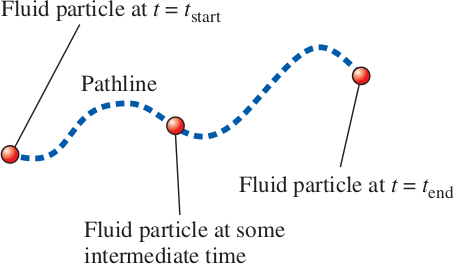
\includegraphics[width=8cm]{pathl}
\caption{Trayectoria de corriente de una particula.}
\label{pathl}
\end{figure}

\begin{equation}
\vec{x} = \vec{x}_{start} + \int_{t_{start}}^t \vec{V} dt
\label{patl}
\end{equation}
donde $x_{start}$ es la posicion inicial de la particula trazadora en el tiempo inicial $t_{start}$. Si el campo de velocidades es permanente, las particulas de fluido siguen las lineas de flujo y estas son identicas a las trayectorias de corriente. 

\emph{Particle image velocimetry (PIV)} es una tecnica para medir la velocidad de un campo de flujo. PIV usa peque\~nas particulas suspendidas en el flujo como trazadores las cuales son iluminadas con luz laser para determinar la posicion y direccion de cada una de ellas en un instante de tiempo.

\subsection{Lineas de trazos}
Si insertamos un pequeno tubo dentro de un fluido e introducimos un  trazador continuo dentro del fluido, la curva que forma las diferentes particulas trazadoras liberadas en intervalo de tiempo constante son la \textbf{linea de trazos} (ver figura~\ref{litra}). Note que en la figura~\ref{litra}, el numero sobre la particula indica el orden en que fueron liberadas dentro del fluido. 
% Fig 4-23 Cengel 
\begin{figure}[h]
\centering
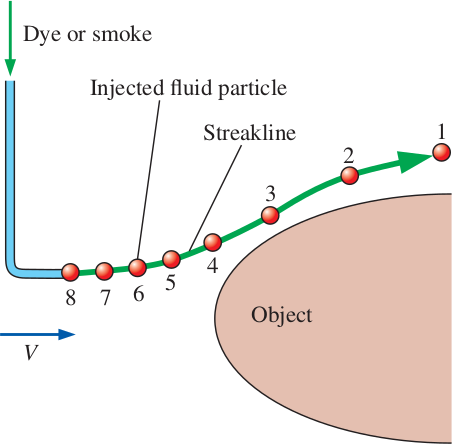
\includegraphics[width=8cm]{litra}
\caption{Line de trazos formada por la inyeccion continua de un trazador en un fluido.}
\label{litra}
\end{figure}
Mientras que en \emph{flujo permanente}, las \emph{lineas de flujo}, las \emph{trayectorias de corriente} y las \emph{lineas de trazos} son iguales, en \emph{flujo no permanente} estas no coinciden. La principal diferencia es que las lineas de flujo son patrones instantaneos de flujo mientras que las lineas de trazos es una foto del patron promedio del flujo en un invervalo de tiempo y las trayectorias de corriente son el recorrido de una particula en un intervalo de tiempo. 

% WE NEED VIDEOS TO EXPLAIN THE DIFERENCES

En un campo de flujo conocido, la linea de trazos puede conocerse a partir de la inyeccion continua de un trazador en un fluido desde un tiempo inicial de la inyeccion $t_{inject}$ hasta un tiempo actual $t_{present}$ utilizando la ecuacion~\ref{patl} as:
\begin{equation}
\vec{x} = \vec{x}_{injection} + \int_{t_{inject}}^{t_{present}} \vec{V} dt
\label{trazl}
\end{equation}


\subsection{Lineas de tiempo}
Las \textbf{lineas de tiempo} son representadas por particulas adjacentes para $t_0$  cuya linea se va deformando a lo largo del flujo gracias al campo de velocidades y la friccion con las paredes (ver figura~\ref{linet}). Estas son importantes para examinar la uniformidad del flujo. 
% Fig 4-28 Cengel 
\begin{figure}[h]
\centering
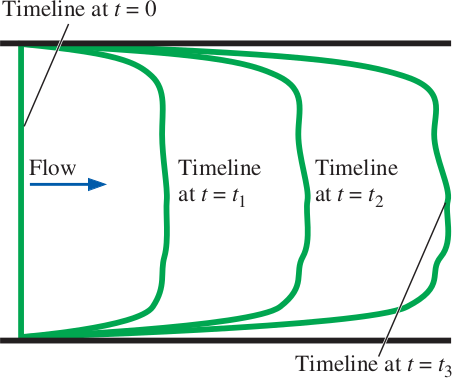
\includegraphics[width=8cm]{linet}
\caption{Linea de tiempo formada por particulas que se deforma en el tiempo debido al campo de flujo.}
\label{linet}
\end{figure}

\section{Tipos de movimiento o deformaci\'on de un elemento de fluido}
Un elemento de fluido puede estar sometido a cuatro tipos de movimiento o deformaci\'on:\textbf{traslaci\'on}, \textbf{rotaci\'on}, \textbf{deformaci\'on lineal} y \textbf{deformaci\'on cortante} (ver figura~\ref{tmove}). El estudio de la dinamica de fluidos es complicado ya que estos tipos de movimiento ocurren muchas veces simultaneamente. Estos tipos de movimiento son descritos en terminos de tasas (en matematicas, velocidad y sus derivadas): \emph{velocidad} (tasa de traslaci\'on), \emph{velocidad angular} (tasa de rotaci\'on), \emph{tasa de deformaci\'on lineal}, \emph{tasa de deformaci\'on cortante}.

% Fig 4-35 Cengel 
\begin{figure}[h]
\centering
\includegraphics[width=8cm]{tmove}
\caption{Tipos de movimiento o deformacion de un fluido: a) traslaci\'on, b) rotaci\'on, c) deformaci\'on lineal y d) deformaci\'on cortante.}
\label{tmove}
\end{figure}

\begin{itemize}
\item[Vector de la tasa de traslacion o vector velocidad]
$$
\vec{V}=u\vec{i}+v\vec{j}+w\vec{k}
$$

$\vec{V}$ describr el desplazamiento de un elemento de una posicion ($x,y,z$) a otra.

\item[Tasa de rotacion (velocidad angular)] en un punto es definida como la tasa de rotacion promedio de dos lineas perpendiculares que se intersectan en dicho punto. Consideremos la figura~\ref{rotat} en donde un elemento en 2D rota, se traslada y se deforma. En el tiempo $t_1$,  las lineas $a$ y $b$ se intersectan perpendicularmente en el punto $P$ en el plano $xy$. Cuando el elemento se mueve y rota en un intervalo $dt=t_2 - t_1$, en el timepo $t_2$ la linea $a$ rota un angulo $\alpha_a$ y la linea $b$ rota $\alpha_b$, ambos angulos son positivos porque ellos rotan en contra de las manecillas del reloj. El angulo promedio de rotacion en $dt$ es por lo tanto $(\alpha_a +\alpha_b)/2$. La tasa de rotacion  o velocidad angular $\omega$ es entonces la derivada con respecto a $t$ de el angulo promedio como:
% Fig 4-36 Cengel 
\begin{figure}[h]
\centering
\includegraphics[width=8cm]{rotat}
\caption{Rotacio, traslacion y deformacion de un elemento de fluido en 2D. Definicion de la rotaci\'on en el punto $P$.}
\label{rotat}
\end{figure}

$$
\omega = \frac{d}{dt}\left( \frac{\alpha_a + \alpha_b}{2} \right) = \frac{1}{2} \left( \frac{\partial v}{\partial x}-\frac{\partial u}{\partial y}




\end{itemize}
\end{document}
